%============================================================
% 02_body.tex — 본문
%
% 이 파일에 논문 본문을 작성합니다.
% 아래 내용은 사용 방법을 안내하는 예시이므로,
% 내용을 확인한 뒤 지우고 실제 논문을 작성하세요.
%
% 섹션 구조:
%   \section{제목}           → I. 제목  (로마 숫자 자동)
%   \subsection{제목}        → 1. 제목
%   \subsubsection{제목}     → 1.1. 제목
%============================================================


%------------------------------------------------------------
\section{서론}
%------------------------------------------------------------

\jiwon[2]
% \jiwon[숫자]는 한글 더미 텍스트입니다 (Lorem ipsum의 한글 버전).
% 위 줄을 지우고 서론을 작성하세요.


%------------------------------------------------------------
\section{이론적 배경 및 선행연구 조사}\label{sec:search}
%------------------------------------------------------------
% \label{이름}을 붙이면 본문 어디서든 \ref{이름}으로 해당 번호를 참조할 수 있습니다.

\subsection{소제목}
\subsubsection{과학영재 창의연구(R\&E)}
% R\&E 처럼 특수문자 &는 앞에 \를 붙여야 합니다.

\jiwon[6-7]

앞서 \ref{sec:search}절에서 본 바와 같이 이론적 배경은 매우 어렵다.
% \ref{sec:search}는 위의 \label{sec:search}가 붙은 절 번호를 자동으로 가져옵니다.


%------------------------------------------------------------
% [그림 삽입 예시]
% images/ 폴더에 그림 파일을 넣은 뒤 아래와 같이 삽입합니다.
%------------------------------------------------------------

\begin{figure}[!ht]
  \centering
  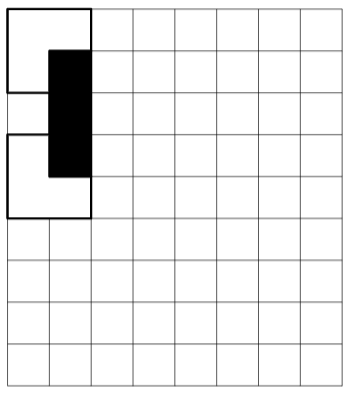
\includegraphics[width=.15\textwidth]{images/B(8, 9).png}
  % width=.15\textwidth → 텍스트 폭의 15%. 크기를 자유롭게 조절하세요.
  \caption{bad pair of $9\times 8$ deficient tile}
  % \caption{} 안에 그림 설명을 씁니다.
  \label{fig:my_label}
  % \label{}로 이름을 붙이면 본문에서 그림 \ref{fig:my_label}로 참조할 수 있습니다.
\end{figure}


%------------------------------------------------------------
% [정리류 환경 예시]
% 사용 가능한 환경: theorem(정리), lemma(보조정리), corollary(따름정리),
%                   definition(정의), example(보기), remark(참고)
%------------------------------------------------------------

\begin{definition}
  정의란 무엇일까? \citep{aanjaneya2009tromino, golomb2021polyominoes, nitica2017tilings}
  % \citep{키}로 참고문헌을 인용합니다. 키는 refs.bib 파일에 정의되어 있습니다.
  % 여러 문헌을 동시에 인용할 때는 쉼표로 구분합니다.
\end{definition}

\jiwon[3-4]

\begin{theorem}\label{thm:what}
  정리란 무엇일까?
\end{theorem}


%------------------------------------------------------------
\subsection{그림 삽입 방법}
%------------------------------------------------------------

아래에서는 그림을 삽입하는 방법을 안내한다. 크게 두 가지 방법이 있다.
\begin{enumerate}[(a)]
  \item 그림 파일을 images 폴더에 업로드 한 후, 그 파일을 넣는 방식.
  \item 텍을 이용하여 직접 그림을 그리는 방식.
\end{enumerate}
그러나, 어느 방식이든, 그림의 위치를 \TeX에게 맡기려면, figure 환경을 이용해야한다.
또 하나의 팁을 주자면, 그림파일을 미리 준비하지 않았더라도, \TeX이 갖고 있는 예시그림을 이용하여
그림의 위치를 미리 어느 정도 살펴볼 수 있다는 것이다.

다음 예시는 \TeX이 갖고 있는 그림예제를 이용하여 그림을 삽입해 본 것이다.

\begin{figure}[!ht]
  \centering
  \includegraphics[width=.4\textwidth]{example-image}
  % example-image는 TeX이 기본 제공하는 예시 그림입니다.
  % 실제 사용할 때는 images/파일명.png 처럼 직접 준비한 파일로 교체하세요.
  \caption{이 그림의 캡션은?!}
  \label{fig:my_fig_label}
\end{figure}

figure 환경에 넣은 그림에는 각 그림에 label을 지정해두었으므로, 상호참조 기능을 이용하여
``그림 \ref{fig:my_label}\을 참고하라.''와 같이 해당 그림을 언급할 수 있다.

한가지 유의할 점은, 논문에서 그림은 필요한 경우에만 넣는다는 것이다. 다시 말해, 논문에
그림을 넣는 것은 논문의 내용에 (상호참조 등을 통해) 그 그림이 언급될 때만 가능한 것으로
여기는 것이 일반적이다. 따라서 논문에 등장하는 모든 그림은 figure 환경에 넣는 것이 바람직하다 하겠다.


%------------------------------------------------------------
\subsection{표 삽입 방법}
%------------------------------------------------------------

한편 표를 삽입하는 방법은 그림을 삽입하는 방법과 거의 동일하다. figure 환경을 table환경으로
바꾸기만 하면 된다.

\begin{table}[!ht]
  \centering
  \caption{이 표의 캡션은?!}
  % 표의 캡션은 표 위에 옵니다 (\caption을 \begin{tblr} 앞에 두세요).
  \label{tab:my_label}
  \begin{tblr}{hlines, vlines}
    % hlines: 가로선, vlines: 세로선 모두 표시
         & 위치 & 장소 \\
    1    &      &      \\
    2    &      &      \\
    3    &      &      \\
  \end{tblr}
\end{table}

한편 표 \ref{tab:my_booktablabel}에서 볼 수 있는 표 양식은 여러 타이포그라피 교과서에서
권장하는 양식이며, 서구권에서 표준적으로 사용하는 양식이라 할 수 있다.
\begin{table}[!ht]
  \centering
  \caption{예쁜 표의 캡션은?!}
  \label{tab:my_booktablabel}
  \begin{booktabs}{colspec={cccc}}
    % booktabs 환경은 가로선만 있는 깔끔한 표를 만듭니다.
    \toprule
    Case & Box A & Box B & Remarks \\
    \midrule
    \SetCell[r=2]{c,m} A & $+X$ & $-1.0$ & \SetCell[r=2]{c,m} B \\
    \cmidrule[lr]{2-3}
    & $-X$ & $-7.9$ & \\
    \bottomrule
  \end{booktabs}
\end{table}


%------------------------------------------------------------
\subsection{수식 입력 방법}
%------------------------------------------------------------

이번에는 수식을 작성하는 몇 가지 예를 살펴보자. 수식은 크게 두 가지 모드로 작성한다.
\begin{itemize}
  \item 행중수식: 문단 안에 $처럼$ 달러 기호로 감싸 쓰는 수식 \quad 예: $E = mc^2$
  \item 행간수식: 별도의 줄에 \verb|\[ ... \]|로 감싸 쓰는 수식
\end{itemize}

\begin{itemize}
  \item 아래첨자: $A_{b+c}$ (cf. $A_a+b$). 곱하기는 $a\times b$.

  \item 최대정수함수 — \verb|\left|·\verb|\right|로 괄호 크기를 내용에 맞게 조절합니다.
    \[ \left\lfloor \frac{\pi^2}{6}\right\rfloor \]

  \item 분수: $\frac{2}{3}$ \quad 행간수식에서는 분수가 크게 표시됩니다.
    \[ \frac{df}{dt}=\frac{df}{ds}\frac{ds}{dt} \]

  \item 부등호: $1\leq 3\leq 5 \geq 2$.

  \item 여러 줄 정렬 수식 — \verb|&|는 정렬 기준, \verb|\\|은 줄바꿈입니다.
    \begin{align*}
      a & \equiv b \mod{p} \\
      a & \equiv b \pmod{p}
    \end{align*}
\end{itemize}


%------------------------------------------------------------
\section{결론}
%------------------------------------------------------------

\jiwon[4]
% ↑ 지우고 결론을 작성하세요.
